% Chương 2

\chapter{CƠ SỞ LÝ THUYẾT DÙNG ĐỂ GIẢI QUYẾT BÀI TOÁN} 

\label{Chapter2}

\section{Mạng neural tích chập (Convolutional Neural Network - CNN)}

\subsection{Khái niệm}

Mạng neural tích chập (Convolutional Neural Network - CNN) là một loại mạng neural sử dụng trong lĩnh vực xử lý ảnh và nhận dạng. Nó sử dụng các lớp tích chập để trích xuất đặc trưng từ ảnh đầu vào và áp dụng các lớp kết nối đầy đủ để phân loại ảnh. 

\begin{figure}[h!]
	\centering
	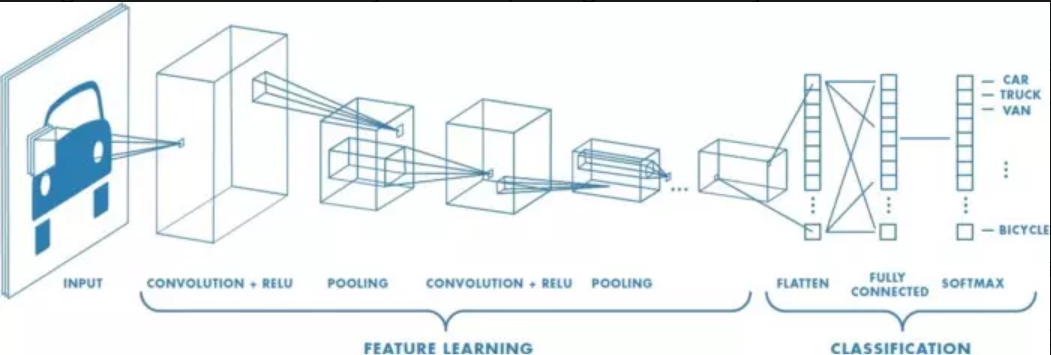
\includegraphics[width=0.8\textwidth]{CNN.png}
	\caption[Toàn bộ luồng CNN để xử lý hình ảnh đầu vào và phân loại các đối tượng dựa trên giá trị.]{Toàn bộ luồng CNN để xử lý hình ảnh đầu vào và phân loại các đối tượng dựa trên giá trị.}
	\label{fig:CNN} 
\end{figure}

Về kỹ thuật, mô hình CNN để training và kiểm tra, mỗi hình ảnh đầu vào sẽ chuyển nó qua 1 loạt các lớp tích chập với các bộ lọc (Kernel), tổng hợp lại các lớp được kết nối đầy đủ (Full Connected) và áp dụng hàm Softmax để phân loại đối tượng có giá trị xác suất giữa 0 và 1. Hình dưới đây là toàn bộ luồng CNN để xử lý hình ảnh đầu vào và phân loại các đối tượng dựa trên giá trị.

\begin{figure}[h!]
	\centering
	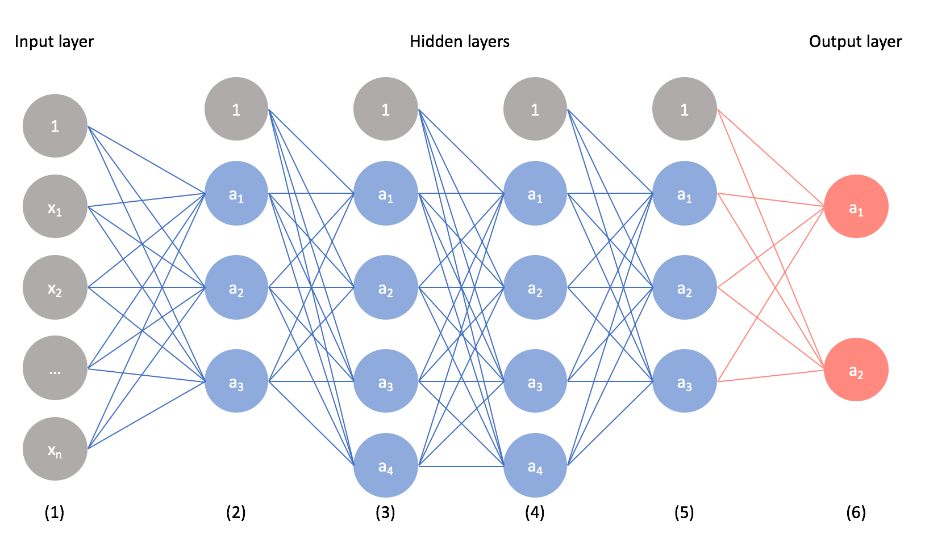
\includegraphics[width=0.7\textwidth]{anh2.png}
	\caption[Mô hình cấu trúc của mạng CNN.]{Mô hình cấu trúc của mạng CNN.}
	\label{fig:anh2} 
\end{figure}

\subsection{Feature trong CNN}

Các feature (đặc trưng) được sử dụng để trích xuất thông tin từ ảnh đầu vào. Các feature này được học tự động từ dữ liệu và được sử dụng để giảm thiểu số lượng thông tin cần xử lý trong quá trình huấn luyện mạng. 

Các feature này có thể là các đường cạnh, các vùng sáng tối, các đường cong và các đối tượng phức tạp hơn. 

Các feature này được trích xuất thông qua các bộ lọc tích chập và được kết hợp lại để tạo thành các feature maps, đóng vai trò quan trọng trong việc phân loại ảnh. Các feature maps này được đưa vào các lớp kết nối đầy đủ để phân loại ảnh đầu vào.

\subsection{Những lớp cơ bản của mạng CNN}

\subsubsection{Convolutional Layer}

Phần quan trọng nhất của toàn mạng CNN, các yếu tố quan trọng trong lớp Convolutional là: padding, stride, feature map và filter map.

\begin{itemize}
	\item Mạng CNN sử dụng filter để áp dụng vào các vùng của ma trận hình ảnh. Các filter map là các ma trận 3 chiều, bên trong đó là những tham số và chúng được gọi là parameters.
	
	\item Stride: dịch chuyển filter map theo từng pixel dựa vào các giá trị từ trái qua phải.
	
	\item Padding: Giá trị viền xung quanh của ma trận hình ảnh sẽ được gán các giá trị 0 để có thể tiến hành nhân tích chập ma trận mà không làm giảm kích thước ma trận ảnh ban đầu.
	
	\item Feature map: Biểu diễn kết quả sau mỗi lần feature map quét qua ma trận ảnh đầu vào. Sau mỗi lần quét thì lớp Convolutional sẽ tiến hành tính toán.
\end{itemize}

\begin{figure}[h!]
	\centering
	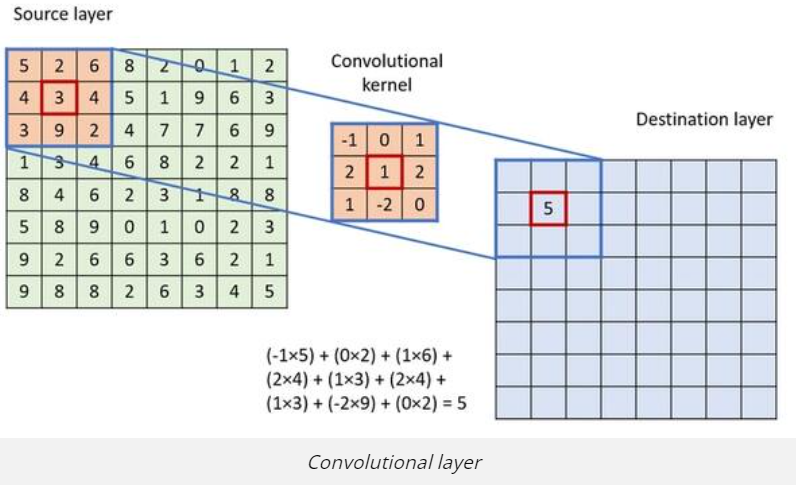
\includegraphics[width=0.7\textwidth]{convolution.png}
	\caption[Convolutional Layer.]{Convolutional Layer.}
	\label{fig:convolution} 
\end{figure}

\subsubsection{ReLU Layer}

Lớp ReLU là hàm kích hoạt trong mạng CNN, được coi là activation function. Nó có tác dụng mô phỏng những nơ ron có tỷ lệ truyền xung qua axon và hỗ trợ tính toán nhanh hơn.

Trong quá trình dùng hàm ReLU, chú ý đến việc tùy chỉnh learning rate và dead unit. Những lướp ReLU được dùng sau khi filter map được tính và áp dụng ReLU lên các giá trị của filter map.

\subsubsection{Pooling Layer}

Khi ma trận ảnh đầu vào có kích thước quá lớn, các lớp Pooling layer sẽ được đặt vào giữa những lớp Convolutional để làm giảm những parameters. Hai loại Pooling được sửu dụng phổ biến: Max pooling và Average.

\subsubsection{Fully Connected Layer}

Lớp có nhiệm vụ đưa ra kết quả sau khi 2 lớp Convolutional và Pooling đã nhận được ảnh truyền, khi này, ta sẽ thu được một model đọc được thông tin của ảnh.

\subsection{Kiến trúc của mạng CNN}

Mạng CNN là tập hợp những Convolutional layer xếp chồng lên nhau, đồng thời mạng sử dụng những hàm như ReLU và Tanh để kích hoạt các trọng số trong các node. Các lớp này sau khi qua các hàm activation sẽ có trọng số trong những node và có thể tạo ra những thông tin trừu tượng hơn đến với các lớp kế tiếp trong mạng.  

Cấu trúc cơ bản của một mô hình CNN:

\begin{itemize}
	\item Local receptive: Lớp này sử dụng để tách lọc dữ liệu, thông tin hình ảnh để từ đó có thể lựa chọn các vùng có giá trị sử dụng hiệu quả cao nhất.
	
	\item Shared weights field: Lớp này hỗ trợ làm giảm các tham số đến mức tối thiểu trong mạng CNN. Trong từng lớp convolution sẽ chứa các feature map riêng và từng feature thì sẽ có khả năng phát hiện một vài feature trong hình ảnh.
	
	\item Pooling layer: Lớp cuối cùng và sử dụng để làm đơn giản các thông tin output. Sau khi tính toán xong và quét qua các layer trong mạng thì pooling layer sẽ được dùng để lược bỏ các thông tin không hữu ích.
\end{itemize}

\section{Các thư viện được sử dụng}

\subsubsection{Thư viện Numpy}

Thư viện NumPy (Numerical Python) là một thư viện Python phổ biến được sử dụng để làm việc với mảng đa chiều và các phép toán số học trên chúng. NumPy cung cấp một cấu trúc dữ liệu mảng mạnh mẽ và các hàm tiện ích để thực hiện các phép toán số học, xử lý mảng và thao tác trên dữ liệu số.

Dưới đây là một số khái niệm và tính năng chính của NumPy:

\begin{itemize}
	\item Mảng NumPy (ndarray): Mảng NumPy là cấu trúc dữ liệu chính trong NumPy, cho phép lưu trữ và xử lý các mảng đa chiều. Mảng NumPy có kích thước cố định và các phần tử trong mảng cùng kiểu dữ liệu.
	
	\item Các phép toán số học: NumPy cung cấp các hàm và toán tử cho phép thực hiện các phép toán số học trên mảng như cộng, trừ, nhân, chia, lũy thừa, căn bậc hai, logarit...
	
	\item Truy cập phần tử: Bạn có thể truy cập và thay đổi giá trị các phần tử trong mảng NumPy bằng cách sử dụng chỉ mục và cắt mảng (slicing).
	
	\item Hàm toán học và thống kê: NumPy cung cấp nhiều hàm toán học và thống kê tiện ích như min, max, mean, sum, std,... để thao tác trên mảng.
	
	\item Hàm điều kiện: NumPy cung cấp các hàm và phương thức cho phép kiểm tra và lựa chọn các phần tử trong mảng dựa trên các điều kiện như np.where, np.logical$\_$and, np.logical$\_$or,...
	
	\item Thao tác trên mảng: NumPy cung cấp các hàm và phương thức để thực hiện các phép biến đổi mảng như reshape, transpose, flatten, concatenate,...
	
	\item Tích hợp C/C++: NumPy cho phép tích hợp mã C/C++ vào mã Python thông qua giao diện C API của nó, giúp tăng tốc độ xử lý các phép toán số học.
	
	\item NumPy được sử dụng rộng rãi trong nhiều lĩnh vực như khoa học dữ liệu, máy học, tính toán khoa học, xử lý ảnh và âm thanh, mô phỏng vật lý,... Thư viện này là một phần quan trọng của hệ sinh thái Python cho tính toán số và xử lý dữ liệu.
\end{itemize}

\subsubsection{Thư viện OpenCV}

Thư viện cv2 (OpenCV) là một thư viện mã nguồn mở được sử dụng rộng rãi trong xử lý ảnh và thị giác máy tính trong ngôn ngữ lập trình Python. OpenCV cung cấp nhiều chức năng và công cụ mạnh mẽ để xử lý, phân tích và trực quan hóa ảnh và video. Dưới đây là một số chức năng chính của thư viện cv2:

\begin{itemize}
	\item Đọc và ghi ảnh và video: OpenCV cung cấp các hàm để đọc và ghi các tệp tin ảnh và video từ các nguồn khác nhau, bao gồm ổ đĩa, camera,...
	
	\item Xử lý ảnh: OpenCV cung cấp nhiều chức năng để xử lý ảnh, bao gồm chuyển đổi màu sắc, cắt, xoay, thu phóng, lật, v.v. Bạn cũng có thể áp dụng các bộ lọc, làm mờ, lọc nhiễu, phát hiện cạnh và nhiều phép biến đổi khác cho ảnh.
	
	\item Xử lý video: OpenCV hỗ trợ xử lý video, bao gồm khung hình theo thời gian, trích xuất khung hình, ghi lại video và áp dụng các hiệu ứng video.
	
	\item Xử lý thị giác máy tính: OpenCV cung cấp các chức năng và thuật toán để phân tích và nhận dạng các đối tượng trong ảnh, bao gồm nhận dạng khuôn mặt, phát hiện vật thể, trích xuất đặc trưng, theo dõi đối tượng,...
	
	\item Xử lý điểm ảnh: OpenCV cho phép bạn truy cập và chỉnh sửa các điểm ảnh trực tiếp, bao gồm xử lý pixel, tạo hiệu ứng đồ họa và thực hiện các phép tính điểm ảnh phức tạp.
	
	\item Hiển thị ảnh: OpenCV cung cấp các chức năng để hiển thị ảnh và video trực tiếp trên màn hình, tạo cửa sổ đồ họa và tương tác với ảnh.
\end{itemize}

Thư viện cv2 có tính ổn định, tốc độ xử lý nhanh và rất phổ biến trong cộng đồng xử lý ảnh và thị giác máy tính.

\subsubsection{Thư viện Tensorflow}

Thư viện TensorFlow là một thư viện mã nguồn mở phát triển bởi Google AI và được sử dụng rộng rãi trong lĩnh vực học máy và trí tuệ nhân tạo. TensorFlow cung cấp một cấu trúc dữ liệu gọi là "đồ thị tính toán" (computational graph) để biểu diễn và thực thi các phép tính toán số trên dữ liệu. Đồ thị tính toán trong TensorFlow bao gồm các nút (nodes) đại diện cho các phép tính toán và các cung (edges) đại diện cho luồng dữ liệu giữa các nút. Dưới đây là một số khái niệm và tính năng chính của TensorFlow:

\begin{itemize}
	\item Đồ thị tính toán (Computational graph): TensorFlow sử dụng đồ thị tính toán để biểu diễn và thực thi các phép tính toán. Đồ thị tính toán giúp tối ưu hóa và tận dụng được tính song song của phần cứng để thực hiện các phép tính nhanh chóng.
	
	\item Tensors: TensorFlow sử dụng cấu trúc dữ liệu tensor để lưu trữ và xử lý dữ liệu. Tensor có thể là một vector, ma trận, hay một mảng đa chiều với các phần tử cùng kiểu dữ liệu.
	
	\item Các lớp và phép tính: TensorFlow cung cấp một loạt các lớp và phép tính để xây dựng các mô hình học máy. Các lớp bao gồm các lớp mạng nơ-ron, lớp tích chập, lớp tổng hợp, lớp tái tạo,... Phép tính bao gồm các phép tính toán như cộng, trừ, nhân, chia, lũy thừa,...
	
	\item Tối ưu hóa và tạo mô hình: TensorFlow cung cấp các tối ưu hóa để tối đa hóa hiệu suất và tăng tốc độ huấn luyện mô hình. Ngoài ra, TensorFlow cũng cung cấp khả năng tạo và lưu trữ các mô hình đã huấn luyện để sử dụng sau này.
	
	\item Tích hợp và mở rộng: TensorFlow cho phép tích hợp và mở rộng với các công cụ và thư viện khác như Keras, scikit-learn, OpenCV, v.v. Điều này giúp thực hiện các tác vụ phức tạp và kết hợp các công cụ và thuật toán khác nhau.
	
	\item Tính tương thích và di động: TensorFlow hỗ trợ nhiều phiên bản và cung cấp tính tương thích đa nền tảng, cho phép chạy trên các thiết bị di động, máy tính cá nhân, máy chủ, và cụm máy tính phân tán.
\end{itemize}

TensorFlow là một công cụ mạnh mẽ trong lĩnh vực học máy và trí tuệ nhân tạo, cho phép xây dựng và huấn luyện các mô hình phức tạp và giải quyết các bài toán thực tế.

\subsubsection{Thư viện Sklearn}

Scikit-learn, hay còn được gọi là sklearn, là một thư viện mã nguồn mở phổ biến trong ngôn ngữ lập trình Python được sử dụng cho Machine Learning và Data Mining. Scikit-learn cung cấp nhiều công cụ và thuật toán tiện ích để xây dựng và đánh giá các mô hình học máy, phân tích dữ liệu và thực hiện các tác vụ tiền xử lý dữ liệu. Dưới đây là một số chức năng và tính năng chính của thư viện scikit-learn:

\begin{itemize}
	\item Cung cấp các thuật toán học máy tiêu chuẩn: Scikit-learn cung cấp các thuật toán học máy phổ biến như hồi quy tuyến tính, hồi quy logistic, máy vector hỗ trợ (SVM), cây quyết định, Random Forest, K-means clustering,... Các thuật toán này được triển khai một cách hiệu quả và dễ sử dụng.
	
	\item Tích hợp các công cụ tiền xử lý dữ liệu: Scikit-learn cung cấp nhiều công cụ tiền xử lý dữ liệu như chuẩn hóa dữ liệu, mã hóa biến định danh, xử lý giá trị thiếu, trích xuất đặc trưng,... Điều này giúp chuẩn bị dữ liệu cho việc huấn luyện mô hình.
	
	\item Đánh giá và tối ưu hóa mô hình: Scikit-learn cung cấp các phép đo và công cụ để đánh giá hiệu suất của mô hình học máy, bao gồm chia dữ liệu thành tập huấn luyện và tập kiểm tra, cross-validation, tính toán độ chính xác, độ phân loại, mất mát,... Ngoài ra, scikit-learn cũng cung cấp các công cụ tối ưu hóa để điều chỉnh các siêu tham số của mô hình.
	
	\item Tích hợp với các thư viện khác: Scikit-learn tích hợp tốt với các thư viện khác trong hệ sinh thái của Python như NumPy, Pandas và Matplotlib, tạo điều kiện thuận lợi cho xử lý dữ liệu và trực quan hóa kết quả.
\end{itemize}

Scikit-learn là một công cụ mạnh mẽ và phổ biến trong lĩnh vực Machine Learning, đặc biệt là trong các tác vụ phân loại, hồi quy và gom cụm dữ liệu. Với tư cách là một thư viện mã nguồn mở, scikit-learn đang tiếp tục được phát triển và cung cấp cập nhật mới để phục vụ cộng đồng Machine Learning ngày càng lớn.

\subsubsection{Thư viện Matplotlib}

Matplotlib là một thư viện trong Python được sử dụng để tạo và hiển thị đồ thị, biểu đồ, hình ảnh và các loại visualizations khác. Nó cung cấp các công cụ mạnh mẽ để tạo ra các biểu đồ chất lượng cao, giúp bạn trực quan hóa dữ liệu một cách dễ dàng và linh hoạt. Dưới đây là một số thành phần chính trong thư viện matplotlib:

\begin{itemize}
	\item pyplot: Giao diện API cơ bản của Matplotlib, cung cấp các hàm để tạo và tùy chỉnh đồ thị và biểu đồ.
	
	\item Figure: Đại diện cho một hình ảnh hoặc một tệp tin hình ảnh.
	
	\item Axes: Cung cấp các phương thức để tạo các đối tượng đồ thị như các trục, điểm, đường.
	
	\item Subplots: Cho phép tạo và quản lý nhiều đồ thị trong cùng một hình ảnh.
	
	\item Plot: Hàm để tạo các loại đồ thị và biểu đồ, bao gồm đồ thị đường (line plot), biểu đồ cột (bar plot), biểu đồ hộp (box plot), đồ thị điểm (scatter plot).
	
	\item Colorbar: Hiển thị thanh màu để giải thích giá trị của màu sắc trong đồ thị.
	
	\item Title, Label, Legend`: Cung cấp các phương thức để thêm tiêu đề, nhãn và chú giải vào đồ thị.
\end{itemize}

Matplotlib cũng hỗ trợ nhiều kiểu đồ thị và biểu đồ, cho phép bạn tùy chỉnh màu sắc, kích thước, kiểu đường, điểm, các đánh dấu trục, v.v. Thư viện này rất linh hoạt và mạnh mẽ, cho phép bạn tạo ra các visualizations phức tạp và tùy chỉnh chúng theo ý muốn.

\subsubsection{Thư viện Keras}

Keras là một thư viện mã nguồn mở cho Python được sử dụng để xây dựng các mô hình học máy và mạng nơ-ron. Nó được thiết kế để làm cho việc xây dựng mô hình học máy trở nên dễ dàng và nhanh chóng hơn. Keras có nhiều tính năng hữu ích, bao gồm:

\begin{itemize}
	\item Dễ dàng sử dụng: Keras được thiết kế để làm cho việc xây dựng mô hình học máy trở nên dễ dàng và trực quan hơn.
	
	\item Tích hợp với các thư viện tính toán số: Keras hỗ trợ các thư viện tính toán số như TensorFlow, Theano và CNTK, cho phép bạn chọn thư viện tính toán số phù hợp nhất cho dự án của mình.
	
	\item Hỗ trợ nhiều loại mô hình: Keras hỗ trợ nhiều loại mô hình, bao gồm mạng nơ-ron tiêu chuẩn, mạng nơ-ron tích chập và mạng nơ-ron tái tạo.
	
	\item Tích hợp với các công cụ tối ưu hóa: Keras cung cấp các công cụ tối ưu hóa để giúp bạn tìm kiếm các tham số tốt nhất cho mô hình của mình.
	
	\item Hỗ trợ các lớp và hàm kích hoạt tiêu chuẩn: Keras cung cấp các lớp và hàm kích hoạt tiêu chuẩn để giúp bạn xây dựng mô hình học máy nhanh chóng và dễ dàng.
\end{itemize}

Keras là một trong những thư viện phổ biến nhất cho việc xây dựng các mô hình học máy và mạng nơ-ron. 

\section{Mô hình phát hiện khuôn mặt}

Việc sử dụng mô hình phát hiện khuôn mặt có sẵn như ResnetSSD là một cách tiếp cận hiệu quả để nhận dạng và phát hiện khuôn mặt trong các ứng dụng thực tế. Mô hình này được xây dựng trên nền tảng deep learning và có khả năng phát hiện khuôn mặt với độ chính xác cao.

Một số lưu ý khi sử dụng mô hình này là:

\begin{itemize}
	\item Đảm bảo rằng ảnh hoặc video đầu vào đủ lớn và độ phân giải cao để đảm bảo độ chính xác của kết quả phát hiện.
	
	\item Có thể cần điều chỉnh các tham số của mô hình để phù hợp với ứng dụng cụ thể.
	
	\item Để đạt được hiệu quả cao nhất, nên sử dụng mô hình này kết hợp với các công cụ nhận dạng khuôn mặt khác để xác định danh tính của người được phát hiện.
\end{itemize}

Với mô hình phát hiện khuôn mặt ResnetSSD, bạn có thể dễ dàng tích hợp vào các ứng dụng thực tế như hệ thống an ninh, ứng dụng nhận dạng khuôn mặt và nhiều ứng dụng khác.

Trong đề tài này, chúng ta sử dụng một mô hình phát hiện khuôn mặt có sẵn để có thể phát hiện khuôn mặt, từ đó chúng ta có thể dự đoán việc đeo khẩu trang và nhận diện cảm xúc.









